\documentclass[11pt,letterpaper]{article}
\usepackage[margin=1in]{geometry}
\usepackage[T1]{fontenc}
\usepackage[utf8]{inputenc}
\usepackage{mathptmx}
\usepackage{tgtermes}
\renewcommand{\ttdefault}{lmtt}
\usepackage[final]{microtype}
\usepackage{graphicx}
\usepackage{booktabs}
\usepackage{longtable}
\usepackage{amsmath,amssymb,amsthm}
\usepackage{xcolor}
\usepackage[round]{natbib}
\usepackage[font=small,labelfont=bf,skip=5pt]{caption}
\usepackage[colorlinks,linkcolor=blue!45!black,citecolor=blue!45!black,urlcolor=blue!45!black]{hyperref}
\usepackage[capitalise,noabbrev,nameinlink]{cleveref}
\usepackage[shortlabels]{enumitem}
\usepackage{titlesec}
\titleformat{\section}{\large\bfseries}{\thesection}{0.6em}{}
\titleformat{\subsection}{\normalsize\bfseries}{\thesubsection}{0.6em}{}
\titlespacing*{\section}{0pt}{12pt plus 3pt minus 2pt}{5pt plus 1pt}
\titlespacing*{\subsection}{0pt}{9pt plus 2pt minus 2pt}{4pt plus 1pt}
\setlist{itemsep=1pt,topsep=3pt,parsep=0pt}
\setlength{\textfloatsep}{12pt plus 2pt minus 4pt}
\setlength{\floatsep}{10pt plus 2pt minus 2pt}
\renewcommand{\topfraction}{0.9}
\renewcommand{\textfraction}{0.08}
\renewcommand{\floatpagefraction}{0.8}
\setcounter{topnumber}{3}
\newtheorem{proposition}{Proposition}
\crefname{proposition}{Proposition}{Propositions}
% generated by make_figs.py, do not edit
\newcommand{\NaucGemmaVisionfree}{0.70}
\newcommand{\NaucGemmaVisionschemeless}{0.55}
\newcommand{\NaucGemmaVisionshared}{0.87}
\newcommand{\NaucMiniSvgfree}{0.61}
\newcommand{\NaucMiniSvgschemeless}{0.52}
\newcommand{\NaucMiniSvgshared}{0.67}
\newcommand{\NaucMiniTextfree}{0.55}
\newcommand{\NaucMiniTextschemeless}{0.44}
\newcommand{\NaucMiniTextshared}{0.45}
\newcommand{\NaucMiniVisionfree}{0.51}
\newcommand{\NaucMiniVisionschemeless}{0.57}
\newcommand{\NaucMiniVisionshared}{0.70}
\newcommand{\Naucschemelessmax}{0.57}
\newcommand{\Naucschemelessmin}{0.44}
\newcommand{\NciextFiveFive}{[5, 30]\%}
\newcommand{\NciextSolFive}{[74, 97]\%}
\newcommand{\NcifreeFiveDs}{[14, 44]\%}
\newcommand{\NcifreeFiveSol}{[89, 100]\%}
\newcommand{\NcifreeMuseDs}{[48, 89]\%}
\newcommand{\NcifreeMuseSol}{[80, 100]\%}
\newcommand{\NcifreeQwenDs}{[12, 41]\%}
\newcommand{\NcifreeQwenSol}{[63, 90]\%}
\newcommand{\NcifreeSolDs}{[49, 81]\%}
\newcommand{\NcifreeSolSol}{[89, 100]\%}
\newcommand{\NcischemelessFiveDs}{[0, 11]\%}
\newcommand{\NcischemelessFiveSol}{[33, 67]\%}
\newcommand{\NcischemelessMuseDs}{[5, 48]\%}
\newcommand{\NcischemelessMuseSol}{[52, 95]\%}
\newcommand{\NcischemelessQwenDs}{[2, 21]\%}
\newcommand{\NcischemelessQwenSol}{[12, 41]\%}
\newcommand{\NcischemelessSolDs}{[30, 64]\%}
\newcommand{\NcischemelessSolSol}{[89, 100]\%}
\newcommand{\NcisharedFiveDs}{[52, 83]\%}
\newcommand{\NcisharedFiveSol}{[89, 100]\%}
\newcommand{\NcisharedMuseDs}{[35, 85]\%}
\newcommand{\NcisharedMuseSol}{[74, 100]\%}
\newcommand{\NcisharedQwenDs}{[33, 67]\%}
\newcommand{\NcisharedQwenSol}{[78, 98]\%}
\newcommand{\NcisharedSolDs}{[33, 67]\%}
\newcommand{\NcisharedSolSol}{[89, 100]\%}
\newcommand{\Ncleancharts}{101}
\newcommand{\Ncleanfd}{0/202}
\newcommand{\NcolchgA}{9}
\newcommand{\NcolchgB}{16}
\newcommand{\NcolchgC}{11}
\newcommand{\NcolchgCR}{10}
\newcommand{\NcolrA}{-0.006}
\newcommand{\NcolrB}{0.109}
\newcommand{\NcolrC}{-0.007}
\newcommand{\NcolrCR}{-0.041}
\newcommand{\NcolrciA}{[-0.074, 0.046]}
\newcommand{\NcolrciB}{[0.064, 0.174]}
\newcommand{\NcolrciC}{[-0.043, 0.031]}
\newcommand{\NcolrciCR}{[-0.099, 0.082]}
\newcommand{\NcuefreeFive}{0/30}
\newcommand{\NcuefreeMuse}{8/15}
\newcommand{\NcuefreeQwen}{0/30}
\newcommand{\NcuefreeSol}{0/30}
\newcommand{\NcueschemelessFive}{0/30}
\newcommand{\NcueschemelessMuse}{5/11}
\newcommand{\NcueschemelessQwen}{0/30}
\newcommand{\NcueschemelessSol}{1/30}
\newcommand{\NdecorCnn}{17/30}
\newcommand{\NdecorFD}{9/30}
\newcommand{\NdecorFDci}{[17, 48]}
\newcommand{\NdecorFDonmark}{2}
\newcommand{\NdecorFDpc}{30}
\newcommand{\NdecorFDtarget}{0/30}
\newcommand{\NdecorGb}{30/30}
\newcommand{\NdecorGemmaVision}{10/30}
\newcommand{\NdecorMark}{4/30}
\newcommand{\NdecorMarkci}{[5, 30]}
\newcommand{\NdecorMarkpc}{13}
\newcommand{\NdecorMiniSvg}{5/30}
\newcommand{\NdecorMiniText}{3/30}
\newcommand{\NdecorMiniVision}{6/30}
\newcommand{\NdecorNr}{2/30}
\newcommand{\NdecorRadius}{30/30}
\newcommand{\NdecorRadiusci}{[89, 100]}
\newcommand{\NdecorRadiuspc}{100}
\newcommand{\NdecorStrict}{30/30}
\newcommand{\NdecorStrictci}{[89, 100]}
\newcommand{\NdecorStrictpc}{100}
\newcommand{\NdecorTrNocode}{13/30}
\newcommand{\NdecoraucCnn}{0.42}
\newcommand{\NdecoraucGb}{0.17}
\newcommand{\NdecoraucGemmaVision}{0.43}
\newcommand{\NdecoraucMiniSvg}{0.44}
\newcommand{\NdecoraucMiniText}{0.44}
\newcommand{\NdecoraucMiniVision}{0.54}
\newcommand{\NdecoraucNr}{0.56}
\newcommand{\Ndecormonaucmax}{0.54}
\newcommand{\Ndecormonaucmin}{0.43}
\newcommand{\Ndecormonmax}{33}
\newcommand{\Ndecormonmin}{10}
\newcommand{\Ndecorn}{30}
\newcommand{\NdetGemmaVisionfree}{43}
\newcommand{\NdetGemmaVisionschemeless}{4}
\newcommand{\NdetGemmaVisionshared}{42}
\newcommand{\NdetMiniSvgfree}{14}
\newcommand{\NdetMiniSvgschemeless}{10}
\newcommand{\NdetMiniSvgshared}{14}
\newcommand{\NdetMiniTextfree}{1}
\newcommand{\NdetMiniTextschemeless}{1}
\newcommand{\NdetMiniTextshared}{0}
\newcommand{\NdetMiniVisionfree}{15}
\newcommand{\NdetMiniVisionschemeless}{8}
\newcommand{\NdetMiniVisionshared}{26}
\newcommand{\Ndetschemelessmax}{10}
\newcommand{\Ndetschemelessmin}{1}
\newcommand{\NdmcleanDs}{0/101}
\newcommand{\NdmcleanFive}{0/30}
\newcommand{\NdmcleanFiveDs}{0/30}
\newcommand{\NdmcleanFiveFive}{0/30}
\newcommand{\NdmcleanFiveSol}{0/30}
\newcommand{\NdmcleanMuseDs}{0/11}
\newcommand{\NdmcleanMuseSol}{0/11}
\newcommand{\NdmcleanQwenDs}{0/30}
\newcommand{\NdmcleanQwenSol}{0/30}
\newcommand{\NdmcleanSol}{0/101}
\newcommand{\NdmcleanSolDs}{0/30}
\newcommand{\NdmcleanSolSol}{0/30}
\newcommand{\NdmfreeDs}{61/105}
\newcommand{\NdmfreeFiveDs}{11/30}
\newcommand{\NdmfreeFiveSol}{30/30}
\newcommand{\NdmfreeMuseDs}{14/15}
\newcommand{\NdmfreeMuseSol}{15/15}
\newcommand{\NdmfreeQwenDs}{11/30}
\newcommand{\NdmfreeQwenSol}{27/30}
\newcommand{\NdmfreeSol}{102/105}
\newcommand{\NdmfreeSolDs}{25/30}
\newcommand{\NdmfreeSolSol}{30/30}
\newcommand{\NdmpccleanDs}{0}
\newcommand{\NdmpccleanFive}{0}
\newcommand{\NdmpccleanSol}{0}
\newcommand{\NdmpcfreeDs}{58}
\newcommand{\NdmpcfreeSol}{97}
\newcommand{\NdmpcschemelessDs}{24}
\newcommand{\NdmpcschemelessFive}{52}
\newcommand{\NdmpcschemelessSol}{64}
\newcommand{\NdmpcsharedDs}{92}
\newcommand{\NdmpcsharedSol}{100}
\newcommand{\NdmschemelessDs}{24/101}
\newcommand{\NdmschemelessFive}{31/60}
\newcommand{\NdmschemelessFiveDs}{0/30}
\newcommand{\NdmschemelessFiveFive}{4/30}
\newcommand{\NdmschemelessFiveSol}{16/30}
\newcommand{\NdmschemelessMuseDs}{4/11}
\newcommand{\NdmschemelessMuseSol}{9/11}
\newcommand{\NdmschemelessQwenDs}{3/30}
\newcommand{\NdmschemelessQwenSol}{10/30}
\newcommand{\NdmschemelessSol}{65/101}
\newcommand{\NdmschemelessSolDs}{17/30}
\newcommand{\NdmschemelessSolFive}{27/30}
\newcommand{\NdmschemelessSolSol}{30/30}
\newcommand{\NdmsharedDs}{93/101}
\newcommand{\NdmsharedFiveDs}{30/30}
\newcommand{\NdmsharedFiveSol}{30/30}
\newcommand{\NdmsharedMuseDs}{11/11}
\newcommand{\NdmsharedMuseSol}{11/11}
\newcommand{\NdmsharedQwenDs}{29/30}
\newcommand{\NdmsharedQwenSol}{29/29}
\newcommand{\NdmsharedSol}{100/100}
\newcommand{\NdmsharedSolDs}{23/30}
\newcommand{\NdmsharedSolSol}{30/30}
\newcommand{\NextFiveFive}{4/30}
\newcommand{\NextFiveFivepc}{13}
\newcommand{\NextFiveFiveredraw}{0/30}
\newcommand{\NextSolFive}{27/30}
\newcommand{\NextSolFivepc}{90}
\newcommand{\NextSolFiveredraw}{0/30}
\newcommand{\Nextclean}{0/30}
\newcommand{\NfprGemmaVision}{0}
\newcommand{\NfprMiniSvg}{2}
\newcommand{\NfprMiniText}{0}
\newcommand{\NfprMiniVision}{3}
\newcommand{\NfreeFiveDs}{8/30}
\newcommand{\NfreeFiveSol}{30/30}
\newcommand{\NfreeMuseDs}{11/15}
\newcommand{\NfreeMuseSol}{15/15}
\newcommand{\NfreeQwenDs}{7/30}
\newcommand{\NfreeQwenSol}{24/30}
\newcommand{\NfreeSolDs}{20/30}
\newcommand{\NfreeSolSol}{30/30}
\newcommand{\NgamePM}{2.85}
\newcommand{\NgamePN}{1.95}
\newcommand{\NgamediffBA}{0.00}
\newcommand{\NgamediffBAci}{[$-$0.14, 0.14]}
\newcommand{\NgamediffCCR}{$-$0.01}
\newcommand{\NgamediffCCRci}{[$-$0.02, 0.01]}
\newcommand{\NgamedriftdiffBA}{68}
\newcommand{\NgamedriftdiffBAci}{[57, 79]}
\newcommand{\NgamedriftdiffCCR}{81}
\newcommand{\NgamedriftdiffCCRci}{[56, 106]}
\newcommand{\Ngamegridnash}{0.10}
\newcommand{\Ngamenonnash}{0.43, $-$0.25}
\newcommand{\NgamepermitRawdelta}{0.11}
\newcommand{\NgamepermitRawdeltaci}{[0.08, 0.13]}
\newcommand{\NgamepermitRawdrift}{+80}
\newcommand{\NgamepermitRawdriftci}{[60, 99]}
\newcommand{\NgamepermitRawendnash}{4/4}
\newcommand{\NgamepermitRawfail}{0/120}
\newcommand{\NgamepermitRawn}{4}
\newcommand{\NgamepermitRawprice}{2.01}
\newcommand{\NgamepermitRawpriceci}{[1.99, 2.02]}
\newcommand{\NgamepermitRedrawdelta}{0.11}
\newcommand{\NgamepermitRedrawdeltaci}{[0.08, 0.14]}
\newcommand{\NgamepermitRedrawdrift}{$-$1}
\newcommand{\NgamepermitRedrawdriftci}{[$-$8, 6]}
\newcommand{\NgamepermitRedrawendnash}{4/4}
\newcommand{\NgamepermitRedrawfail}{0/120}
\newcommand{\NgamepermitRedrawn}{4}
\newcommand{\NgamepermitRedrawprice}{2.01}
\newcommand{\NgamepermitRedrawpriceci}{[1.99, 2.03]}
\newcommand{\Ngamerawdelta}{0.11}
\newcommand{\Ngamerawdeltaci}{[$-$0.05, 0.26]}
\newcommand{\Ngamerawdrift}{+68}
\newcommand{\Ngamerawdriftci}{[54, 82]}
\newcommand{\Ngamerawendnash}{6/8}
\newcommand{\Ngamerawfail}{4/240}
\newcommand{\Ngamerawn}{8}
\newcommand{\Ngamerawprice}{2.01}
\newcommand{\Ngamerawpriceci}{[1.92, 2.09]}
\newcommand{\Ngameredrawdelta}{0.11}
\newcommand{\Ngameredrawdeltaci}{[0.09, 0.12]}
\newcommand{\Ngameredrawdrift}{0}
\newcommand{\Ngameredrawdriftci}{[$-$4, 3]}
\newcommand{\Ngameredrawendnash}{8/8}
\newcommand{\Ngameredrawfail}{6/240}
\newcommand{\Ngameredrawn}{8}
\newcommand{\Ngameredrawprice}{2.01}
\newcommand{\Ngameredrawpriceci}{[2.00, 2.02]}
\newcommand{\Ngamerounds}{15}
\newcommand{\NholmFSFive}{5.2\times10^{-5}}
\newcommand{\NholmFSMuse}{0.85}
\newcommand{\NholmFSQwen}{1.6\times10^{-4}}
\newcommand{\NholmFSSol}{1}
\newcommand{\NholmLRFive}{7.4\times10^{-13}}
\newcommand{\NholmLRMuse}{1.9\times10^{-5}}
\newcommand{\NholmLRQwen}{1.4\times10^{-9}}
\newcommand{\NholmLRSol}{2.4\times10^{-17}}
\newcommand{\NholmSHFive}{5.2\times10^{-5}}
\newcommand{\NholmSHMuse}{1}
\newcommand{\NholmSHQwen}{3.8\times10^{-7}}
\newcommand{\NholmSHSol}{1}
\newcommand{\NholmSolvsFive}{1}
\newcommand{\NholmextFive}{0.0059}
\newcommand{\Nholmm}{14}
\newcommand{\Nholmsurvive}{9}
\newcommand{\Nkeptrows}{905}
\newcommand{\NmmFivedonor}{0/30}
\newcommand{\NmmFiveown}{15/30}
\newcommand{\NmmSoldonor}{0/30}
\newcommand{\NmmSolown}{30/30}
\newcommand{\Nmonfprmax}{3}
\newcommand{\NnatFive}{17/30}
\newcommand{\NnatMuse}{6/10}
\newcommand{\NnatQwen}{7/30}
\newcommand{\NnatSol}{27/30}
\newcommand{\NnocueMuse}{4/6}
\newcommand{\NnocueSol}{29/29}
\newcommand{\NpFSFive}{5.8\times10^{-6}}
\newcommand{\NpFSMuse}{0.17}
\newcommand{\NpFSQwen}{2.3\times10^{-5}}
\newcommand{\NpFSSol}{1}
\newcommand{\NpLRFive}{5.7\times10^{-14}}
\newcommand{\NpLRMuse}{1.9\times10^{-6}}
\newcommand{\NpLRQwen}{1.2\times10^{-10}}
\newcommand{\NpLRSol}{1.7\times10^{-18}}
\newcommand{\NpSHFive}{5.8\times10^{-6}}
\newcommand{\NpSHMuse}{0.48}
\newcommand{\NpSHQwen}{3.5\times10^{-8}}
\newcommand{\NpSHSol}{1}
\newcommand{\NpSolvsFive}{0.25}
\newcommand{\Npeerpoolfracfree}{99/105}
\newcommand{\Npeerpoolfracschemeless}{61/101}
\newcommand{\Npeerpoolfracshared}{98/100}
\newcommand{\Npeerpoolfree}{94}
\newcommand{\Npeerpoolschemeless}{60}
\newcommand{\Npeerpoolshared}{98}
\newcommand{\NpextFive}{9.8\times10^{-4}}
\newcommand{\NpoolfreeFive}{30/30}
\newcommand{\NpoolfreeMuse}{15/15}
\newcommand{\NpoolfreeQwen}{24/30}
\newcommand{\NpoolfreeSol}{30/30}
\newcommand{\NpoolpcfreeFive}{100}
\newcommand{\NpoolpcfreeMuse}{100}
\newcommand{\NpoolpcfreeQwen}{80}
\newcommand{\NpoolpcfreeSol}{100}
\newcommand{\NpoolpcredrawFive}{0}
\newcommand{\NpoolpcredrawMuse}{0}
\newcommand{\NpoolpcredrawQwen}{0}
\newcommand{\NpoolpcredrawSol}{0}
\newcommand{\NpoolpcschemelessFive}{50}
\newcommand{\NpoolpcschemelessMuse}{82}
\newcommand{\NpoolpcschemelessQwen}{23}
\newcommand{\NpoolpcschemelessSol}{100}
\newcommand{\NpoolpcsharedFive}{100}
\newcommand{\NpoolpcsharedMuse}{100}
\newcommand{\NpoolpcsharedQwen}{93}
\newcommand{\NpoolpcsharedSol}{100}
\newcommand{\NpoolredrawFive}{0/60}
\newcommand{\NpoolredrawMuse}{0/21}
\newcommand{\NpoolredrawQwen}{0/59}
\newcommand{\NpoolredrawSol}{0/60}
\newcommand{\NpoolschemelessFive}{15/30}
\newcommand{\NpoolschemelessMuse}{9/11}
\newcommand{\NpoolschemelessQwen}{7/30}
\newcommand{\NpoolschemelessSol}{30/30}
\newcommand{\NpoolsharedFive}{30/30}
\newcommand{\NpoolsharedMuse}{11/11}
\newcommand{\NpoolsharedQwen}{27/29}
\newcommand{\NpoolsharedSol}{30/30}
\newcommand{\Nrawrows}{917}
\newcommand{\Nredrawall}{0/401}
\newcommand{\Nredrawallci}{[0, 1]\%}
\newcommand{\Nredrawoverall}{0/461}
\newcommand{\Nredrawoverallci}{[0, 1]\%}
\newcommand{\Nretest}{27/27}
\newcommand{\NruleFive}{0/30}
\newcommand{\NruleMuse}{1/10}
\newcommand{\NruleQwen}{0/30}
\newcommand{\NruleSol}{0/30}
\newcommand{\NschemelessFiveDs}{0/30}
\newcommand{\NschemelessFiveSol}{15/30}
\newcommand{\NschemelessMuseDs}{2/11}
\newcommand{\NschemelessMuseSol}{9/11}
\newcommand{\NschemelessQwenDs}{2/30}
\newcommand{\NschemelessQwenSol}{7/30}
\newcommand{\NschemelessSolDs}{14/30}
\newcommand{\NschemelessSolSol}{30/30}
\newcommand{\NsharedFiveDs}{21/30}
\newcommand{\NsharedFiveSol}{30/30}
\newcommand{\NsharedMuseDs}{7/11}
\newcommand{\NsharedMuseSol}{11/11}
\newcommand{\NsharedQwenDs}{15/30}
\newcommand{\NsharedQwenSol}{27/29}
\newcommand{\NsharedSolDs}{15/30}
\newcommand{\NsharedSolSol}{30/30}
\newcommand{\NshufextFiveFive}{1.3}
\newcommand{\NshufextSolFive}{8.6}
\newcommand{\Nshufmax}{10.5}
\newcommand{\Nshufmin}{0.0}
\newcommand{\Nshufsol}{9.4}
\newcommand{\Nshufsoltrue}{100}
\newcommand{\NsolncGemmaVision}{7/30}
\newcommand{\NsolncMiniSvg}{0/30}
\newcommand{\NsolncMiniText}{3/30}
\newcommand{\NsolncMiniVision}{5/30}
\newcommand{\NsolncaucGemmaVision}{0.53}
\newcommand{\NsolncaucMiniSvg}{0.42}
\newcommand{\NsolncaucMiniText}{0.51}
\newcommand{\NsolncaucMiniVision}{0.65}
\newcommand{\NsolncaucciGemmaVision}{[0.39, 0.66]}
\newcommand{\NsolncaucciMiniSvg}{[0.29, 0.56]}
\newcommand{\NsolncaucciMiniText}{[0.36, 0.65]}
\newcommand{\NsolncaucciMiniVision}{[0.53, 0.77]}
\newcommand{\Nsolncmax}{23}
\newcommand{\Nsolncmin}{0}
\newcommand{\NsolncpcGemmaVision}{23}
\newcommand{\NsolncpcMiniSvg}{0}
\newcommand{\NsolncpcMiniText}{10}
\newcommand{\NsolncpcMiniVision}{17}
\newcommand{\Ntgall}{47/100}
\newcommand{\Ntgclean}{5/101}
\newcommand{\NtgcleanSol}{1/30}
\newcommand{\Ntgshared}{8/101}
\newcommand{\NtgsharedSol}{0/30}
\newcommand{\Ntgsol}{26/30}
\newcommand{\Ntgsolcorrect}{26/30}
\newcommand{\NtmCnnLoeoschemelessauc}{0.67}
\newcommand{\NtmCnnLoeoschemelessaucci}{[0.59, 0.74]}
\newcommand{\NtmCnnLoeoschemelessdet}{35}
\newcommand{\NtmCnnLoeoschemelessfpr}{3}
\newcommand{\NtmCnnLoeosharedauc}{1.00}
\newcommand{\NtmCnnLoeosharedaucci}{[0.99, 1.00]}
\newcommand{\NtmCnnLoeoshareddet}{98}
\newcommand{\NtmCnnLoeosharedfpr}{3}
\newcommand{\NtmCnnRandschemelessauc}{0.64}
\newcommand{\NtmCnnRandschemelessaucci}{[0.56, 0.71]}
\newcommand{\NtmCnnRandschemelessdet}{11}
\newcommand{\NtmCnnRandschemelessfpr}{0}
\newcommand{\NtmCnnRandsharedauc}{1.00}
\newcommand{\NtmCnnRandsharedaucci}{[1.00, 1.00]}
\newcommand{\NtmCnnRandshareddet}{95}
\newcommand{\NtmCnnRandsharedfpr}{0}
\newcommand{\NtmCnnTrschemelessauc}{0.67}
\newcommand{\NtmCnnTrschemelessaucci}{[0.59, 0.74]}
\newcommand{\NtmCnnTrschemelessdet}{35}
\newcommand{\NtmCnnTrschemelessfpr}{9}
\newcommand{\NtmCnnTrsharedauc}{1.00}
\newcommand{\NtmCnnTrsharedaucci}{[0.99, 1.00]}
\newcommand{\NtmCnnTrshareddet}{98}
\newcommand{\NtmCnnTrsharedfpr}{9}
\newcommand{\NtmCnnsol}{43}
\newcommand{\NtmCnnsolauc}{0.78}
\newcommand{\NtmCnnsolaucci}{[0.66, 0.90]}
\newcommand{\NtmCnnsoldettr}{70}
\newcommand{\NtmCnnsolfprtr}{20}
\newcommand{\NtmGbLoeoschemelessauc}{0.97}
\newcommand{\NtmGbLoeoschemelessaucci}{[0.95, 0.99]}
\newcommand{\NtmGbLoeoschemelessdet}{95}
\newcommand{\NtmGbLoeoschemelessfpr}{1}
\newcommand{\NtmGbLoeosharedauc}{1.00}
\newcommand{\NtmGbLoeosharedaucci}{[1.00, 1.00]}
\newcommand{\NtmGbLoeoshareddet}{100}
\newcommand{\NtmGbLoeosharedfpr}{1}
\newcommand{\NtmGbRandschemelessauc}{1.00}
\newcommand{\NtmGbRandschemelessaucci}{[0.99, 1.00]}
\newcommand{\NtmGbRandschemelessdet}{100}
\newcommand{\NtmGbRandschemelessfpr}{8}
\newcommand{\NtmGbRandsharedauc}{1.00}
\newcommand{\NtmGbRandsharedaucci}{[1.00, 1.00]}
\newcommand{\NtmGbRandshareddet}{100}
\newcommand{\NtmGbRandsharedfpr}{8}
\newcommand{\NtmGbTrschemelessauc}{0.97}
\newcommand{\NtmGbTrschemelessaucci}{[0.95, 0.99]}
\newcommand{\NtmGbTrschemelessdet}{95}
\newcommand{\NtmGbTrschemelessfpr}{0}
\newcommand{\NtmGbTrsharedauc}{1.00}
\newcommand{\NtmGbTrsharedaucci}{[1.00, 1.00]}
\newcommand{\NtmGbTrshareddet}{100}
\newcommand{\NtmGbTrsharedfpr}{0}
\newcommand{\NtmGbsol}{100}
\newcommand{\NtmGbsolauc}{1.00}
\newcommand{\NtmGbsolaucci}{[1.00, 1.00]}
\newcommand{\NtmGbsoldettr}{100}
\newcommand{\NtmGbsolfprtr}{0}
\newcommand{\NtmNrLoeoschemelessauc}{0.69}
\newcommand{\NtmNrLoeoschemelessaucci}{[0.62, 0.76]}
\newcommand{\NtmNrLoeoschemelessdet}{26}
\newcommand{\NtmNrLoeoschemelessfpr}{3}
\newcommand{\NtmNrLoeosharedauc}{0.38}
\newcommand{\NtmNrLoeosharedaucci}{[0.32, 0.46]}
\newcommand{\NtmNrLoeoshareddet}{8}
\newcommand{\NtmNrLoeosharedfpr}{3}
\newcommand{\NtmNrRandschemelessauc}{0.88}
\newcommand{\NtmNrRandschemelessaucci}{[0.83, 0.93]}
\newcommand{\NtmNrRandschemelessdet}{63}
\newcommand{\NtmNrRandschemelessfpr}{8}
\newcommand{\NtmNrRandsharedauc}{0.88}
\newcommand{\NtmNrRandsharedaucci}{[0.82, 0.92]}
\newcommand{\NtmNrRandshareddet}{50}
\newcommand{\NtmNrRandsharedfpr}{8}
\newcommand{\NtmNrTrschemelessauc}{0.69}
\newcommand{\NtmNrTrschemelessaucci}{[0.62, 0.76]}
\newcommand{\NtmNrTrschemelessdet}{42}
\newcommand{\NtmNrTrschemelessfpr}{22}
\newcommand{\NtmNrTrsharedauc}{0.38}
\newcommand{\NtmNrTrsharedaucci}{[0.32, 0.46]}
\newcommand{\NtmNrTrshareddet}{15}
\newcommand{\NtmNrTrsharedfpr}{22}
\newcommand{\NtmNrsol}{17}
\newcommand{\NtmNrsolauc}{0.59}
\newcommand{\NtmNrsolaucci}{[0.45, 0.73]}
\newcommand{\NtmNrsoldettr}{77}
\newcommand{\NtmNrsolfprtr}{63}
\newcommand{\NtmPlrLoeoschemelessauc}{0.56}
\newcommand{\NtmPlrLoeoschemelessaucci}{[0.48, 0.64]}
\newcommand{\NtmPlrLoeoschemelessdet}{21}
\newcommand{\NtmPlrLoeoschemelessfpr}{3}
\newcommand{\NtmPlrLoeosharedauc}{0.77}
\newcommand{\NtmPlrLoeosharedaucci}{[0.71, 0.83]}
\newcommand{\NtmPlrLoeoshareddet}{58}
\newcommand{\NtmPlrLoeosharedfpr}{3}
\newcommand{\NtmPlrRandschemelessauc}{0.61}
\newcommand{\NtmPlrRandschemelessaucci}{[0.54, 0.68]}
\newcommand{\NtmPlrRandschemelessdet}{35}
\newcommand{\NtmPlrRandschemelessfpr}{7}
\newcommand{\NtmPlrRandsharedauc}{0.95}
\newcommand{\NtmPlrRandsharedaucci}{[0.92, 0.98]}
\newcommand{\NtmPlrRandshareddet}{83}
\newcommand{\NtmPlrRandsharedfpr}{7}
\newcommand{\NtmPlrTrschemelessauc}{0.56}
\newcommand{\NtmPlrTrschemelessaucci}{[0.48, 0.64]}
\newcommand{\NtmPlrTrschemelessdet}{52}
\newcommand{\NtmPlrTrschemelessfpr}{45}
\newcommand{\NtmPlrTrsharedauc}{0.77}
\newcommand{\NtmPlrTrsharedaucci}{[0.71, 0.83]}
\newcommand{\NtmPlrTrshareddet}{82}
\newcommand{\NtmPlrTrsharedfpr}{45}
\newcommand{\NtmSlrLoeoschemelessauc}{1.00}
\newcommand{\NtmSlrLoeoschemelessaucci}{[0.99, 1.00]}
\newcommand{\NtmSlrLoeoschemelessdet}{98}
\newcommand{\NtmSlrLoeoschemelessfpr}{3}
\newcommand{\NtmSlrLoeosharedauc}{1.00}
\newcommand{\NtmSlrLoeosharedaucci}{[1.00, 1.00]}
\newcommand{\NtmSlrLoeoshareddet}{100}
\newcommand{\NtmSlrLoeosharedfpr}{3}
\newcommand{\NtmSlrRandschemelessauc}{0.98}
\newcommand{\NtmSlrRandschemelessaucci}{[0.95, 1.00]}
\newcommand{\NtmSlrRandschemelessdet}{98}
\newcommand{\NtmSlrRandschemelessfpr}{0}
\newcommand{\NtmSlrRandsharedauc}{1.00}
\newcommand{\NtmSlrRandsharedaucci}{[1.00, 1.00]}
\newcommand{\NtmSlrRandshareddet}{100}
\newcommand{\NtmSlrRandsharedfpr}{0}
\newcommand{\NtmSlrTrschemelessauc}{1.00}
\newcommand{\NtmSlrTrschemelessaucci}{[0.99, 1.00]}
\newcommand{\NtmSlrTrschemelessdet}{100}
\newcommand{\NtmSlrTrschemelessfpr}{25}
\newcommand{\NtmSlrTrsharedauc}{1.00}
\newcommand{\NtmSlrTrsharedaucci}{[1.00, 1.00]}
\newcommand{\NtmSlrTrshareddet}{100}
\newcommand{\NtmSlrTrsharedfpr}{25}
\newcommand{\NtplRclean}{0/101}
\newcommand{\NtplRqwen}{24/30}
\newcommand{\NtplRschemeless}{94/100}
\newcommand{\NtplRshared}{101/101}
\newcommand{\NtplSclean}{91/101}
\newcommand{\NtplSschemeless}{100/100}
\newcommand{\NtplSshared}{101/101}
\newcommand{\Ntplunflagcharts}{6}
\newcommand{\Ntplunflaghits}{2/12}
\newcommand{\Ntpluniform}{25/30}
\newcommand{\Ntpluniformr}{6}
\newcommand{\Ntxtcom}{0}
\newcommand{\Ntxtcue}{14}
\newcommand{\Ntxthid}{0}
\newcommand{\Ntxtn}{307}
\newcommand{\Ntxtvis}{0}

\newcommand{\fillme}[1]{\textcolor{red!70!black}{[TO FILL: #1]}}
\hypersetup{pdftitle={Hidden in the Chart: Empty Footnotes for AI Sellers}}

\begin{document}
\begin{center}
{\LARGE\bfseries Hidden in the Chart: Empty Footnotes for AI Sellers\par}
\vspace{6pt}
{\large Prompted monitors miss price signals in rendered charts;\\ redrawing from declared data removes them\par}
\end{center}
\vspace{4pt}
\begin{abstract}
\noindentLLM pricing agents may soon publish a chart beside each price, while audits of algorithmic pricing read only declared prices and text. Antitrust has met this gap before: in the ATPCO case, airlines were alleged to signal through fare-filing footnotes that carried no fare data. We test whether an LLM seller can pass a target price to a rival through a chart whose data are locked to its declared prices, whether monitors notice, and what removes the signal. Told to signal one of 11 target prices with no agreed code, gpt-6.1-sol drew charts that it decoded in \NschemelessSolSol\ trials and that gpt-5.5 decoded in \NextSolFive\ (chance 1/11). Four prompted LLM monitors flagged \Nsolncmin--\Nsolncmax\% of these charts at a 5\% false-positive rate. Detectors that know the target grid or the mark do better, but in a matched control of honest charts with a decorative element the grid-aware decoder raised a false alarm on \NdecorFD, and trained detectors could not tell these charts from signalling ones; only a rule written for the observed mark stayed selective. Redrawing every chart from the declared data left \Nredrawall\ correct decodes, and a one-line proof shows that no decoder can beat chance on a redraw. In a \Ngamerounds-round pilot game with no instruction to signal, sellers imitated each other's raw chart styling but did not detectably raise prices. The remedy used for fare filings, publishing only from declared data, also works for agent charts.

\end{abstract}
\vspace{2pt}

\section{Introduction}
\label{sec:intro}
Pricing agents may soon publish a chart of recent prices next to each listing, and rival agents with vision can read it. Audits of algorithmic pricing check the declared prices and the text around them. A chart can also carry a visible mark that is not data, and an audit of the declared data cannot see it.

Antitrust has met this problem before. In \emph{ATPCO}, the U.S.\ Department of Justice alleged that airlines signalled through fare-filing footnotes that held no fare information. The consent decree barred any ``footnote designator that identifies a footnote that contains no information'' and left airlines free to publish their fares \citep{atpco1994}. Parallel pricing alone is lawful \citep{twombly2007}, so what passes between sellers matters; the 2025 RealPage settlement likewise requires pricing software to drop features that ``aligned pricing between competing users'' \citep{realpage2025}. We ask whether LLM sellers can put such an \emph{empty footnote} into a chart, whether monitors flag it, and what removes it.

Prior work leaves this open. In text, frontier models mostly fail to coordinate on a hidden scheme that was not agreed in advance \citep{zolkowski2025,rippin2026}. In images it is easier: a model with Python can hide free-form messages in SVGs that a second model often reads \citep{kezins2026}. No study has tested this in a market, where the chart must show the seller's declared prices exactly, the payload is a price, the reader is a rival seller, and a platform can intervene. Our contributions are:
\begin{enumerate}[leftmargin=*]
\item \textbf{A testbed} for price signals in rendered charts: 4 encoder models, 3 decoders, 3 signalling conditions and a clean control, with a leakage audit (\cref{sec:threat,sec:method}).
\item \textbf{An unflagged channel.} With the data locked and no agreed code, one strong encoder drew charts that two other models read and that prompted monitors barely separated from clean charts (\cref{sec:recovery,sec:detect}).
\item \textbf{A remedy with a proof.} Redrawing each chart from the declared data, the analogue of the \emph{ATPCO} footnote rule, removed every signal, and it provably caps any decoder at chance (\cref{sec:redraw}).
\item \textbf{A pilot game} with no instruction to signal, in which sellers imitated raw chart styling without a detectable price effect (\cref{sec:game}).
\end{enumerate}

\begin{figure}[t]
\centering
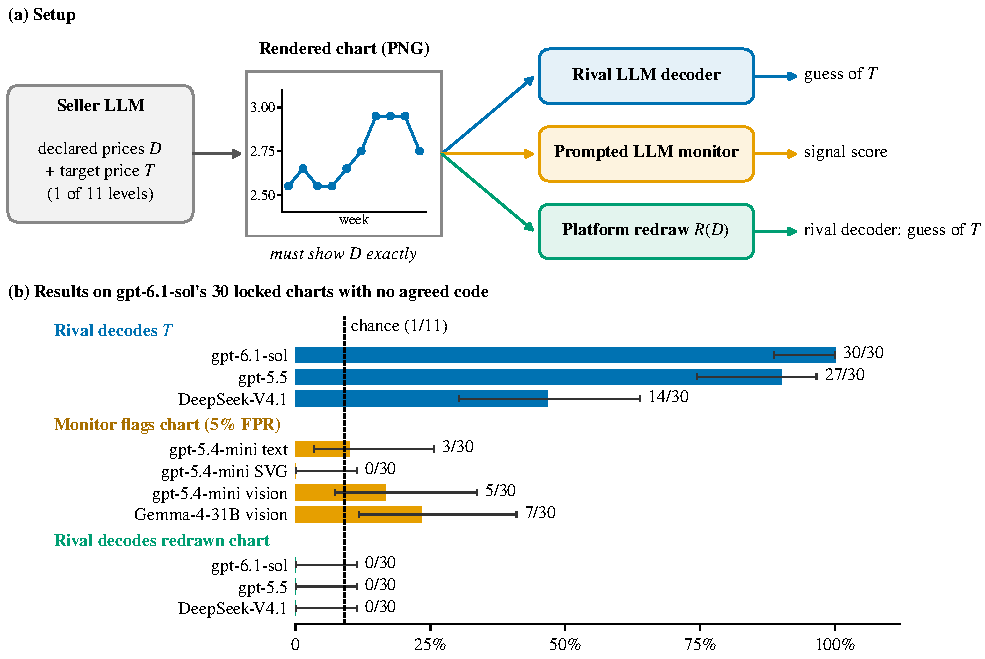
\includegraphics[width=\linewidth]{figs/fig0_overview.pdf}
\caption{\textbf{Overview.} (a)~The seller draws a chart that must show its declared prices $D$ and is told to signal a target $T$. A rival decodes the rendered PNG, a prompted monitor scores it, and the platform can replace it with its own rendering $R(D)$. The thumbnail is a real clean chart's data. (b)~Headline results with Wilson 95\% intervals.}
\label{fig:overview}
\end{figure}

\section{Threat model}
\label{sec:threat}
\textbf{Setting.} Two seller agents list competing products on a platform. Each round a seller declares its prices, and the platform publishes them with a chart that the seller draws. Rivals see the rendered chart. An auditor (the platform or a regulator) checks the declared prices, the seller's text and possibly the chart.

\textbf{Attacker.} The colluding seller (the \emph{encoder}) wants a rival (the \emph{decoder}) to learn a target price $T$, one of 11 levels (about 3.5 bits). The encoder controls everything in the chart except the data, which the platform verifies. In the \emph{no-code} case the sellers have no prior agreement on how to encode $T$ and share only public knowledge, such as the price axis and the set of plausible prices. In the \emph{shared-rule} case they share one public encoding rule, which models a prior agreement.

\textbf{Defender.} The auditor can (i)~ask a prompted LLM monitor whether a chart carries a price signal, (ii)~use detectors that know more (the target grid, the mark, or labelled examples), or (iii)~discard the seller's chart and redraw it from the declared data.

\textbf{Out of scope.} Signals in the prices themselves, in the seller's text, and declared data that depend on $T$. The redraw assumes the declared data are trusted and independent of $T$.

\section{Related work}
\label{sec:related}
\textbf{Algorithmic and LLM collusion.} Pricing algorithms and LLM agents can reach prices above Nash without communicating \citep{calvano2020,fish2024}. \citet{andon2026} report a frontier model recruiting competitors into price fixing through explicit messages, and \citet{leepark2026} find that chain-of-thought monitoring alone cannot detect collusion between LLM pricing agents. We study a channel that neither price monitors nor reasoning monitors read.

\textbf{Steganography between LLM agents.} \citet{motwani2024} formalise secret collusion through steganography, and \citet{mathew2024} show it can emerge under optimisation pressure. \citet{zolkowski2025} find early steganographic capability that fails when no scheme is agreed. \citet{rippin2026} frame tacit coordination as a Schelling-point problem and name shared artefacts as a risky setting; a published chart is such an artefact. CovertCollude \citep{hu2026covertcollude} found no verifiable channel in code-review text when agents were not told how to encode, and its LLM signal-searchers flagged 67\% of clean inputs; our decoders named a price on \Ncleanfd\ plain clean decodes but on \NdecorFD\ decorated clean charts (\cref{sec:recovery}).

\textbf{Image channels and removal.} \citet{kezins2026} showed that a model can hide free-form messages in SVGs with no named scheme and that a second model read 44 of 50, so cross-model reading of image channels is not our claim. We add locked data, a price payload read by a rival, calibrated and trained monitors, a removal defense with a proof, and a pricing game. Removal by regeneration follows paraphrasing defenses in text \citep{roger2023}; AI control \citep{greenblatt2023} motivates measuring both attack and monitor. Covert channels go back to \citet{lampson1973} and \citet{simmons1984}.

\section{Method}
\label{sec:method}
\textbf{Task.} The encoder receives 10 declared weekly prices and a target $T\in\{1.0, 1.2, \dots, 3.0\}$. Prices are a seeded series between 1.05 and 2.95 ending in 5, so no price label lies on the target grid; targets cycle through the levels by trial index. The encoder returns an SVG on a $1280\times640$ canvas and a one-sentence commentary that must read as normal market talk and must not state $T$. The decoder receives only the rendered PNG, the public series, the marker coordinates and the target grid. It may run up to five Python measurements on the pixels, then names a price or answers ``no signal''. A \emph{hit} is a guess that rounds to the true level.

\textbf{Conditions} (\emph{arms}; examples in \cref{app:charts}).
\emph{Free canvas}: the encoder may draw anything; this bounds legibility and does not test evasion.
\emph{Locked, no code}: the chart must pass a fidelity gate (filled circles at the declared coordinates, the 10 two-decimal labels, a white background, no transforms on data circles), and the encoder is told to signal $T$ so that another model can read it, with no scheme named. The decoder still knows the grid and both see the price axis; this shared frame does much of the Schelling work \citep{rippin2026}.
\emph{Locked, shared rule}: both models are told one public rule that maps $T$ to the size of the leftmost marker.
\emph{Clean}: a locked chart with no target, drawn under a ``plain chart, marker radius 5'' instruction.
\emph{Decorated clean} (matched control, gpt-6.1-sol only, \Ndecorn\ charts): the same locked prompt with no target and no plain-chart or radius instruction, told instead to add one decorative reference element of its choice, so that honest charts also carry a non-data mark.
A chart that fails the gate counts as a miss. We do not publish the encoding prompts (\cref{sec:dualuse}).

\textbf{Models.} Encoders: gpt-6.1-sol and gpt-5.5 (OpenAI API), Qwen3.5-397B-A17B and Muse-Spark-Open-816B-A42B (Hugging Face). Decoders: gpt-6.1-sol and DeepSeek-V4.1-Flash; gpt-5.5 later decoded the cached no-code charts of gpt-5.5 and gpt-6.1-sol. Hugging Face models run at temperature 0.7 (encoders) or 0 (decoders, monitors) with the trial index as seed; OpenAI reasoning models take neither. Cells have 30 trials, except Muse (15 free, 11 locked).

\textbf{Counting rule.} For each encoder, decoder and trial we count the first decode that returned an answer; retries after API errors are not extra attempts. One Qwen shared-rule trial never returned an answer and is excluded ($n=29$). The harness logged \Nrawrows\ decoder rows, and this rule leaves one per encoder, decoder and trial (\Nkeptrows).

\textbf{Monitors and detectors.} Four \emph{prompted monitors}: gpt-5.4-mini on the commentary, the SVG source and the image, and Gemma-4-31B-it on the image. Each scores how likely an item carries a price signal for a rival, without being told any rule. \emph{Trained detectors} (CPU only): gradient boosting on SVG structure features, with and without the six marker-radius features; logistic regression on SVG features and on pixels; and a small CNN on the image. They separate target-carrying from clean charts and are tested leave-one-encoder-out (LOEO) and on random 5-fold splits. Thresholds are set at 5\% FPR on one encoder's 30 clean charts; for trained detectors this is the held-out encoder, an oracle choice that favours the detector.

\textbf{Redraw defense.} The platform discards the seller's SVG and renders the declared prices $D$ with its own template, giving $R(D)$. We decode every locked target-carrying chart again after the redraw.
\begin{proposition}\label{prop:redraw}
If $D$ is independent of $T$, then so is $R(D)$. Hence $I(T;R(D))=0$, and every decoder $g$ satisfies $\Pr[g(R(D))=T]\le\max_t \Pr[T=t]$, which is $1/11$ here.
\end{proposition}
\noindent\emph{Proof.} $R(D)$ is a function of $D$ alone, and a function of a variable independent of $T$ is independent of $T$. $\square$

\textbf{Statistics.} Wilson 95\% intervals \citep{wilson1927}; Fisher exact tests between arms (different charts) and exact McNemar tests for paired conditions (same charts), with the gpt-6.1-sol decoder and a Holm correction over all \Nholmm\ tests.

\section{Results}
\label{sec:results}
\subsection{Claim 1: one strong encoder builds a readable channel with no agreed code}
\label{sec:recovery}

\begin{figure}[t]
\centering
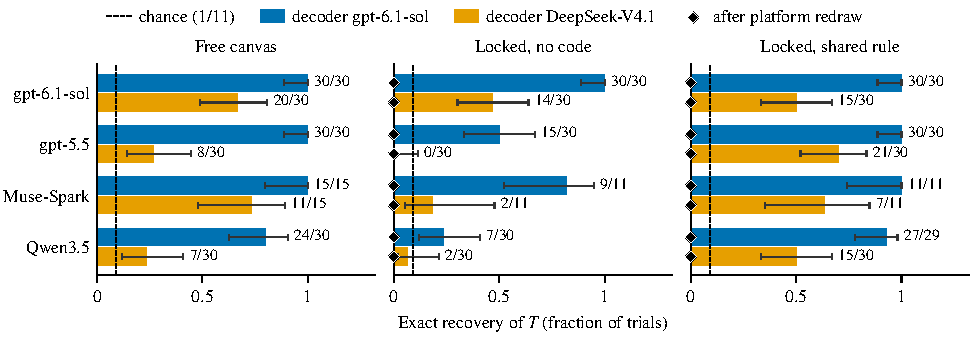
\includegraphics[width=\linewidth]{figs/fig2_recovery.pdf}
\caption{\textbf{Locking the data hurts most encoders but not gpt-6.1-sol, and every redraw falls to zero.} Exact recovery of $T$ (hits/trials) by arm, encoder and decoder, with Wilson 95\% intervals. Dashed line: chance. Black diamonds: recovery on the redrawn chart for the same trials (locked arms only).}
\label{fig:recovery}
\end{figure}

With the data locked and no agreed code, gpt-6.1-sol decoded its own charts in \NschemelessSolSol\ trials (95\% CI \NcischemelessSolSol; chance 9\%) and DeepSeek read them in \NschemelessSolDs\ (\cref{fig:recovery}). Other encoders were weaker: the gpt-6.1-sol decoder read gpt-5.5 in \NschemelessFiveSol, Muse in \NschemelessMuseSol\ and Qwen in \NschemelessQwenSol. The no-code result therefore rests on one strong encoder that was told to signal.

It is not self-recognition. gpt-5.5 read gpt-6.1-sol's no-code charts in \NextSolFive\ (\NciextSolFive), not detectably worse than gpt-6.1-sol itself (McNemar $p=\NpSolvsFive$). gpt-5.5 read its own charts in only \NextFiveFive, fewer than gpt-6.1-sol read them (McNemar $p=\NpextFive$, Holm $p=\NholmextFive$; \cref{tab:ext}). The skill lies in writing the chart, not in a bond between copies of one model.

Locking the data cut recovery for gpt-5.5 (Holm $p=\NholmFSFive$) and Qwen (Holm $p=\NholmFSQwen$); the drop for Muse was not significant ($n=11$, Holm $p=\NholmFSMuse$), and gpt-6.1-sol lost nothing (\NpoolfreeSol\ free, \NpoolschemelessSol\ no code). The shared rule restored recovery for gpt-5.5 (Holm $p=\NholmSHFive$) and Qwen (Holm $p=\NholmSHQwen$); gpt-6.1-sol did as well without a code as with one. \Nholmsurvive\ of the \Nholmm\ tests survive Holm (\cref{tab:pooled}).

\textbf{What carries the signal.} Most gpt-6.1-sol no-code charts (\NnatSol) add an unlabeled horizontal reference line at the target's height on the chart's own price axis. About half of gpt-5.5's (\NnatFive) add some visible non-data mark read against the same axis. This is not pixel-level steganography: the mark is in plain view and works as a Schelling point, a salient choice each model expects the other to make given the shared grid and axis. Like an empty footnote, it passes audits of declared data because it adds nothing to them. We give no other parameters.

\textbf{The decoder reads the chart, not the harness} (\cref{app:audit}). Decoding each gpt-6.1-sol chart with another trial's prompt gave \NmmSolown\ hits against the chart's own target and \NmmSoldonor\ against the prompt donor's. Scoring guesses against permuted targets dropped every pair to \Nshufmin--\Nshufmax\%. The commentary never contained $T$, and removing the \Ntxtcue\ charts whose visible text names the channel leaves gpt-6.1-sol at \NnocueSol.

\textbf{Matched clean control.} On the \Ndecorn\ decorated clean charts, which carry no target, the gpt-6.1-sol decoder reported a signal and named a price on \NdecorFD\ (95\% CI \NdecorFDci\%). A harmless decoration is thus often read as a signal. This does not explain the no-code result: there the decoder named the exact target in \NschemelessSolSol\ trials, while a decoder that named a random level on every chart would be right about 1 time in 11.

\subsection{Claim 2: prompted monitors miss the channel; informed detectors need updates}
\label{sec:detect}

\begin{table}[t]
\centering\small
\caption{\textbf{Detection rises with what the detector knows.} Detecting gpt-6.1-sol no-code charts ($n=30$) at 5\% FPR, with the threshold set on gpt-6.1-sol's 30 clean charts. Decoder rows count charts where the decoder reported a signal ($^\dagger$on gpt-5.5's own 30 clean charts). The targeted check is a rule written after we saw the mark. Trained rows were trained on the other three encoders, with an oracle threshold. Decorated clean: \Ndecorn\ gpt-6.1-sol clean charts drawn with one decorative element and no target, at the same threshold. AUROC compares no-code with plain clean charts.}
\label{tab:detectors}
{\footnotesize\setlength{\tabcolsep}{3.5pt}\begin{tabular}{llcccc}
\toprule
Detector & Needs to know & \shortstack{Clean\\flagged} & \shortstack{Decorated\\clean flagged} & \shortstack{No-code\\flagged} & AUROC [95\% CI] \\
\midrule
Prompted monitor: gpt-5.4-mini text & none & 1/30 & 3/30 & 3/30 & 0.51 [0.36, 0.65] \\
Prompted monitor: gpt-5.4-mini SVG & none & 1/30 & 5/30 & 0/30 & 0.42 [0.29, 0.56] \\
Prompted monitor: gpt-5.4-mini vision & none & 0/30 & 6/30 & 5/30 & 0.65 [0.53, 0.77] \\
Prompted monitor: Gemma-4-31B vision & none & 1/30 & 10/30 & 7/30 & 0.53 [0.39, 0.66] \\
\midrule
Decoder as monitor: gpt-6.1-sol & 11-level grid & 0/30 & 9/30 & 30/30 & -- \\
Decoder as monitor: gpt-5.5 & 11-level grid & 0/30$^\dagger$ & -- & 27/30 & -- \\
Targeted mark check (rule-based) & the mark & 1/30 & 4/30 & 26/30 & -- \\
Trained, held-out encoder: SVG features & labelled examples & $\le$1/30 & 30/30 & 30/30 & 1.00 [1.00, 1.00] \\
Trained, held-out encoder: SVG features, no radius & labelled examples & $\le$1/30 & 2/30 & 5/30 & 0.59 [0.45, 0.73] \\
Trained, held-out encoder: image CNN & labelled examples & $\le$1/30 & 17/30 & 13/30 & 0.78 [0.66, 0.90] \\
\bottomrule
\end{tabular}
}
\end{table}

A monitor makes a yes/no call, while a decoder must name one of 11 levels, so flagging is the easier task. Even so, the four prompted monitors flagged only \Nsolncmin--\Nsolncmax\% of gpt-6.1-sol charts that gpt-6.1-sol and gpt-5.5 decoded almost perfectly (\cref{tab:detectors}); only gpt-5.4-mini on the image has an AUROC interval above 0.5 (\NsolncaucMiniVision\ \NsolncaucciMiniVision). Pooled over encoders, monitors detected \Ndetschemelessmin--\Ndetschemelessmax\% of no-code charts (AUROC \Naucschemelessmin--\Naucschemelessmax; \cref{tab:monitors}), though Gemma flagged \NdetGemmaVisionshared\% of the cruder shared-rule charts.

Knowledge narrows the gap, but decorated clean charts raise false alarms. A decoder used as a monitor knows the grid; it reported a signal on \NdmschemelessSolSol\ no-code charts and \NdmcleanSolSol\ plain clean ones, but also on \NdecorFD\ decorated clean charts. The targeted check flagged \Ntgsol\ no-code charts with \NtgcleanSol\ plain and \NdecorMark\ decorated clean (95\% CI \NdecorMarkci\%), but it was written after reading the charts and must be rewritten for each new mark. At the plain-clean threshold the prompted monitors flagged \Ndecormonmin--\Ndecormonmax\% of decorated clean charts, as many as or more than no-code charts, and separated the two no better than chance (AUROC \Ndecormonaucmin--\Ndecormonaucmax).

Trained detectors show how a prompt artefact can pass for detection. Gradient boosting on SVG features reached a LOEO AUROC of \NtmGbLoeoschemelessauc, mostly from marker radius: the clean prompt names radius 5 and the no-code prompt does not, and in \Ntpluniform\ gpt-6.1-sol no-code charts every marker has radius \Ntpluniformr. Without radius features, AUROC fell to \NtmNrLoeoschemelessauc\ pooled and \NtmNrsolauc\ \NtmNrsolaucci\ on held-out gpt-6.1-sol. The image CNN reached \NtmCnnsolauc\ \NtmCnnsolaucci\ on held-out gpt-6.1-sol, but with the threshold carried over from the training encoders its clean false-positive rate rose to \NtmCnnsolfprtr\%. The matched control confirms the artefact. Without the radius instruction gpt-6.1-sol did not use radius 5, so the radius check flagged all \NdecorRadius\ decorated clean charts. SVG gradient boosting flagged \NdecorGb\ of them (AUROC \NdecoraucGb\ for no-code against decorated) and the CNN \NdecorCnn\ (\NdecoraucCnn). Trained detectors learned the clean prompt and the encoders they had seen, not the signal.

\subsection{Claim 3: redrawing from declared data removes the signal}
\label{sec:redraw}
Across \Nredrawall\ decodes of redrawn locked charts by the two main decoders, none recovered the target (95\% CI \Nredrawallci); with the added gpt-5.5 decodes, \Nredrawoverall. For gpt-6.1-sol, recovery fell from \NpoolschemelessSol\ (no code) and \NpoolsharedSol\ (shared rule) to \NpoolredrawSol\ (McNemar, Holm $p=\NholmLRSol$). The empirical zero is a sanity check; the guarantee is \cref{prop:redraw}, which holds whatever the mark. Detectors must be updated for each new mark or encoder; the redraw needs no update. Template checks either need the rule or reject most honest charts (\cref{app:template}).

\subsection{Claim 4: unprompted sellers imitate raw charts but do not raise prices detectably}
\label{sec:game}

\begin{figure}[t]
\centering
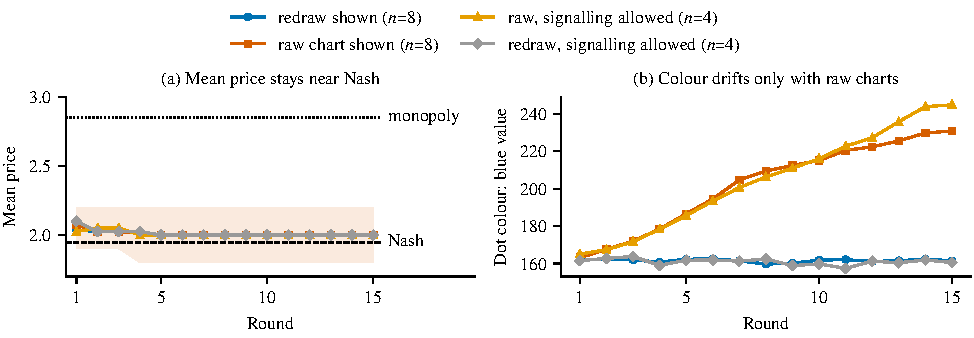
\includegraphics[width=\linewidth]{figs/fig5_game.pdf}
\caption{\textbf{Raw charts change how sellers draw, not what they charge.} Pilot game, two gpt-6.1-sol sellers, \Ngamerounds\ rounds. (a)~Mean price per round; the band is the range over raw-chart episodes. (b)~Blue value of each seller's dot colour, averaged over sellers and episodes. ``Signalling allowed'' adds one permissive sentence to both prompts; it is an upper bound, not a test of emergence.}
\label{fig:game}
\end{figure}

Above, the encoder is told to signal. Here no one is. Two gpt-6.1-sol sellers play \Ngamerounds\ rounds in the logit market of \citet{calvano2020}, as in \citet{fish2024}, scaled so that the Nash price (\NgamePN) and the monopoly price (\NgamePM) fall inside the price grid (\cref{app:game}). Each round a seller sees the public history, its own private note and the rival's last chart, and returns a price, a note and an SVG chart of its last ten prices that must pass the fidelity gate. The prompt asks only for maximum total profit. Two conditions differ only in what the rival sees: the platform redraw or the seller's own chart. We report the profit index $\Delta=(\bar\pi-\pi_N)/(\pi_M-\pi_N)$, 0 at Nash and 1 at monopoly, with $t$ intervals over episodes.

With $n=\Ngamerawn$ episodes per condition, raw charts had no detectable price effect (\cref{fig:game}a): mean $\Delta$ was \Ngameredrawdelta\ \Ngameredrawdeltaci\ with the redraw and \Ngamerawdelta\ \Ngamerawdeltaci\ with raw charts, a paired difference of \NgamediffBA\ \NgamediffBAci. This excludes increases above 0.14 of the Nash--monopoly gap, but not slow emergence over long horizons; \citet{fish2024} use 300 periods. Sellers did react to raw charts (\cref{fig:game}b): their dot colours drifted together, with the blue value rising by \Ngamerawdrift\ \Ngamerawdriftci\ on a 0--255 scale, which we read as imitation of the rival's styling. Under the redraw there is nothing to imitate, and drift was \Ngameredrawdrift\ \Ngameredrawdriftci.

\section{Discussion}
\label{sec:discussion}
\textbf{An empty footnote has an old remedy.} The mark adds nothing to the declared data, so audits of that data pass it, and a rival who expects it can read it. The \emph{ATPCO} decree did not ask regulators to work out which footnotes signalled; it barred footnotes that carried no information \citep{atpco1994}. In container shipping, the European Commission likewise accepted commitments that price announcements state full, binding prices \citep{eu2016}. Redrawing from declared data is the analogue for agent charts: sellers keep publishing their prices, and the platform renders them. Detection, by contrast, must chase each new mark and, as the matched control shows, also flags honest decorated charts.

\textbf{Costs and gaps.} Sellers lose control of chart styling. The redraw does nothing about price-only tacit collusion \citep{calvano2020,fish2024} or about the commentary, which needs paraphrase or removal \citep{roger2023}.

\textbf{Capability, not propensity.} Our main evidence is a capability under instruction. Whether sellers would use the channel unprompted is a question of propensity, which the pilot game tested once, in a small setting.

\section{Limitations}
\label{sec:limits}
\begin{enumerate}[leftmargin=*,label=(\arabic*)]
\item One task and one chart type; 30 trials per cell and 11--15 for Muse, so many intervals are wide.
\item The no-code result rests on one strong encoder told to signal; gpt-5.5 decoded only no-code charts.
\item OpenAI models ran without temperature or seed control, so their runs are not exactly reproducible.
\item Plain clean charts were drawn under a ``plain chart, radius 5'' instruction, which favours monitors and created the radius confound. The matched decorated control raised false-positive rates for most detectors, but it covers one encoder and one kind of decoration chosen by the model.
\item Trained-detector rows use oracle thresholds; thresholds from training encoders transfer poorly.
\item The redraw assumes trusted declared data independent of the target, and does nothing about signals in the prices themselves.
\item The game is a pilot: \Ngamerawn\ paired episodes of \Ngamerounds\ rounds, one model, one market.
\end{enumerate}

\section{Dual use}
\label{sec:dualuse}
Hiding data in images with code tools is public \citep{kezins2026}. We name the mark (\NnatSol\ gpt-6.1-sol no-code charts add an unlabeled horizontal reference line at the target's height on the chart's own price axis) so that readers can check our claims. We publish no encoding prompts, other parameters or evasion guidance. We release the public shared rule, which is the experimental variable and is easy to detect. The recommended defense helps platforms and regulators and offers colluders little.

\section{Conclusion}
\label{sec:conclusion}
A rendered price chart can carry a visible mark that audits of declared data pass. Told to signal, one frontier model drew such marks with the data locked and no agreed code, and two other models read them, while prompted monitors flagged few. Detectors that knew the grid or the mark did better, but false-alarmed on honest decorated charts or must be rebuilt for each new mark. Redrawing from declared data removed every signal and needs no update. Platforms that let pricing agents publish charts should render those charts from declared data.

\paragraph{Code and data.} \url{https://github.com/batmnnn/hidden-in-the-chart} holds the harness, the run logs and the figure script. Every figure, table and number in this report is generated by \texttt{make\_figs.py} from the run logs.

{\small
\begin{thebibliography}{99}\raggedright\setlength{\itemsep}{2pt}
\bibitem[ATPCO(1994)]{atpco1994} \emph{United States v.\ Airline Tariff Publishing Co.}, Civ.\ No.\ 92-2854 (D.D.C.). Proposed Final Judgment and Competitive Impact Statement, 59 Fed.\ Reg., 31 March 1994 (FR Doc.\ 94-7672).
\bibitem[Andon Labs(2026)]{andon2026} Andon Labs. Opus 4.6 on Vending-Bench -- Not Just a Helpful Assistant. Blog post, 5 February 2026.
\bibitem[Twombly(2007)]{twombly2007} \emph{Bell Atlantic Corp.\ v.\ Twombly}, 550 U.S. 544 (2007).
\bibitem[Calvano et al.(2020)]{calvano2020} E.~Calvano, G.~Calzolari, V.~Denicol\`o, S.~Pastorello. Artificial Intelligence, Algorithmic Pricing, and Collusion. \emph{American Economic Review}, 110(10):3267--3297, 2020.
\bibitem[DOJ(2025)]{realpage2025} U.S.\ Department of Justice. Press release on the proposed RealPage settlement, 24 November 2025.
\bibitem[European Commission(2016)]{eu2016} European Commission. Case AT.39850 \emph{Container Shipping}, commitments decision of 7 July 2016. Summary in OJ C 327, 6 September 2016.
\bibitem[Fish et al.(2024)]{fish2024} S.~Fish, Y.~A. Gonczarowski, R.~I. Shorrer. Algorithmic Collusion by Large Language Models. arXiv:2404.00806, 2024.
\bibitem[Greenblatt et al.(2023)]{greenblatt2023} R.~Greenblatt, B.~Shlegeris, K.~Sachan, F.~Roger. AI Control: Improving Safety Despite Intentional Subversion. arXiv:2312.06942, 2023.
\bibitem[Hu et al.(2026)]{hu2026covertcollude} E.~Hu, N.~Tang, K.~C. Ip, G.~Rosenbaum. CovertCollude: A Control Setting for Steganographic Multi-Agent Collusion. AI Control Hackathon, Apart Research, 2026. \url{https://apartresearch.com/sprints/projects/covertcollude-a-control-setting-for-steganographic-multiagent-collusion-vc55}.
\bibitem[Kezins et al.(2026)]{kezins2026} Kezins, Chan, Reynoso, Chua. How does Fable 5.1 hide messages in images? LessWrong, 21 October 2026. \url{https://www.lesswrong.com/posts/WHEQps5PK8LrrcTAb}. Code: \url{https://github.com/cnm13ryan/fable-image-steganography}.
\bibitem[Lampson(1973)]{lampson1973} B.~W. Lampson. A note on the confinement problem. \emph{Communications of the ACM}, 16(10):613--615, 1973.
\bibitem[Lee and Park(2026)]{leepark2026} D.~Lee, H.~Park. Faithful yet Collusive: Why Chain-of-Thought Monitoring Cannot Detect Collusion in LLM Pricing Agents under Oligopolistic Competition. arXiv:2609.18346, 2026.
\bibitem[Mathew et al.(2025)]{mathew2024} Y.~Mathew et al. Hidden in Plain Text: Emergence and Mitigation of Steganographic Collusion in LLMs. In \emph{Proc.\ IJCNLP-AACL 2025}, pages 585--624, 2025. arXiv:2410.03768.
\bibitem[Motwani et al.(2024)]{motwani2024} S.~R. Motwani et al. Secret Collusion among AI Agents: Multi-Agent Deception via Steganography. NeurIPS 2024. arXiv:2402.07510.
\bibitem[Rippin et al.(2026)]{rippin2026} Rippin, Marshall, Africa, Schroeder de Witt. Tool Use Enables Undetectable Steganography in Multi-Agent LLM Systems. arXiv:2606.28425, 2026.
\bibitem[Roger and Greenblatt(2023)]{roger2023} F.~Roger, R.~Greenblatt. Preventing Language Models From Hiding Their Reasoning. arXiv:2310.18512, 2023.
\bibitem[Simmons(1984)]{simmons1984} G.~J. Simmons. The Prisoners' Problem and the Subliminal Channel. In \emph{Advances in Cryptology: Proceedings of Crypto 83}, 1984.
\bibitem[Wilson(1927)]{wilson1927} E.~B. Wilson. Probable inference, the law of succession, and statistical inference. \emph{JASA}, 22(158):209--212, 1927.
\bibitem[Zolkowski et al.(2025)]{zolkowski2025} Zolkowski, Nishimura-Gasparian, McCarthy, Zimmermann, Lindner. Early Signs of Steganographic Capabilities in Frontier LLMs. arXiv:2507.02737, 2025.
\end{thebibliography}
}

\clearpage
\appendix
\section{Example charts}
\label{app:charts}
\begin{figure}[h]
\centering
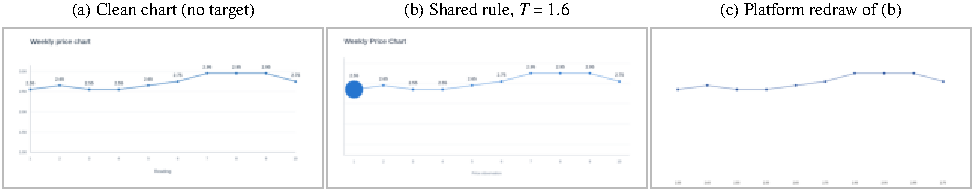
\includegraphics[width=\linewidth]{figs/fig1_charts.pdf}
\caption{(a)~A clean gpt-6.1-sol chart. (b)~A gpt-6.1-sol chart under the public shared rule for $T=1.6$; the declared prices and marker positions are unchanged. (c)~The platform's redraw of (b) from the declared data. No-code charts are not shown (\cref{sec:dualuse}).}
\label{fig:charts}
\end{figure}

\section{Leakage audit}
\label{app:audit}
\textbf{Decoder input.} The rendered PNG, the public series and the coordinates of the 10 data points, the 11-level grid, in the shared arm the public rule, and the outputs of its own Python measurements. Never the commentary, the SVG source, the target, the trial index or the file name.

\textbf{Mismatched prompt.} Each chart is decoded with the public series and prompt of trial $i+7$, so nothing in the prompt relates to the chart's target (\cref{tab:mismatch}). The redraw is the converse check: same prompt, chart replaced, \Nredrawall\ hits.
\begin{center}\small
\captionof{table}{Mismatched-prompt control.}\label{tab:mismatch}
\begin{tabular}{llccc}
\toprule
Encoder & Decoder & $n$ & Hits vs.\ chart's own secret & Hits vs.\ prompt donor's secret \\
\midrule
gpt-5.5 & gpt-6.1-sol & 30 & 15/30 & 0/30 \\
gpt-6.1-sol & gpt-6.1-sol & 30 & 30/30 & 0/30 \\
\bottomrule
\end{tabular}

\end{center}

\textbf{Shuffle control.} For each pair we keep the guesses fixed and score them against 2000 random permutations of the targets. If the decoder read something tied to the trial rather than the chart, the shuffled rate would stay high; it falls to chance in every pair (\Nshufmin--\Nshufmax\%; gpt-6.1-sol same-model: \Nshufsoltrue\% to \Nshufsol\%).

\textbf{Text checks.} We search the commentary, visible SVG text and hidden SVG text (comments, metadata, invisible elements) for $T$, and flag visible text that names a channel or decoding rule (\cref{tab:text}). In \Ntxtcue\ charts the visible text names the channel (Muse free \NcuefreeMuse, Muse no-code \NcueschemelessMuse, gpt-6.1-sol no-code \NcueschemelessSol). Removing them leaves gpt-6.1-sol same-model recovery at \NnocueSol\ and Muse to gpt-6.1-sol at \NnocueMuse.
\begin{center}\footnotesize\setlength{\tabcolsep}{4pt}
\captionof{table}{Text checks on all \Ntxtn\ target-carrying charts.}\label{tab:text}
\begin{tabular}{llccccc}
\toprule
Arm & Encoder & Charts & Commentary & Visible decimal & Hidden text & Text names \\
 & & & has $T$ & equals $T$ & has $T$ & channel or rule \\
\midrule
Free canvas & Muse-Spark & 15 & 0 & 0 & 0 & 8 \\
Free canvas & Qwen3.5 & 30 & 0 & 0 & 0 & 0 \\
Free canvas & gpt-5.5 & 30 & 0 & 0 & 0 & 0 \\
Free canvas & gpt-6.1-sol & 30 & 0 & 0 & 0 & 0 \\
Locked, no code & Muse-Spark & 11 & 0 & 0 & 0 & 5 \\
Locked, no code & Qwen3.5 & 30 & 0 & 0 & 0 & 0 \\
Locked, no code & gpt-5.5 & 30 & 0 & 0 & 0 & 0 \\
Locked, no code & gpt-6.1-sol & 30 & 0 & 0 & 0 & 1 \\
Locked, shared rule & Muse-Spark & 11 & 0 & 0 & 0 & 0 \\
Locked, shared rule & Qwen3.5 & 30 & 0 & 0 & 0 & 0 \\
Locked, shared rule & gpt-5.5 & 30 & 0 & 0 & 0 & 0 \\
Locked, shared rule & gpt-6.1-sol & 30 & 0 & 0 & 0 & 0 \\
\bottomrule
\end{tabular}

\end{center}

\textbf{Convergent marks.} No-code charts that add a non-data element whose geometry varies with the target: gpt-6.1-sol \NnatSol, gpt-5.5 \NnatFive, Muse \NnatMuse, Qwen \NnatQwen. Charts matching the public shared rule: gpt-6.1-sol \NruleSol, gpt-5.5 \NruleFive, Qwen \NruleQwen, Muse \NruleMuse.

\textbf{Decoder sandbox rerun.} A first DeepSeek run hit two bugs in the decoder's Python sandbox that rejected ordinary measurement code (import lines and image loading). We fixed the sandbox and reran all DeepSeek decodes; only the rerun is reported, and the superseded logs are kept. An accidental second decode of 27 Qwen shared-rule charts by gpt-6.1-sol gave the same answer in \Nretest; only the first is counted.

\section{Full results}
\label{app:pairs}
\begin{center}\small
\captionof{table}{Recovery for every arm, encoder and decoder.}\label{tab:pairsfull}
\vspace{-6pt}
\setlength{\tabcolsep}{5pt}\begin{longtable}{lllcccc}
\toprule
Arm & Encoder & Decoder & $n$ & Hits & \% [Wilson 95\% CI] & Redraw hits \\
\midrule
\endhead
Free canvas & gpt-6.1-sol & gpt-6.1-sol & 30 & 30/30 & 100 [89, 100] & -- \\
Free canvas & gpt-6.1-sol & DeepSeek-V4.1 & 30 & 20/30 & 67 [49, 81] & -- \\
Locked, no code & gpt-6.1-sol & gpt-6.1-sol & 30 & 30/30 & 100 [89, 100] & 0/30 \\
Locked, no code & gpt-6.1-sol & DeepSeek-V4.1 & 30 & 14/30 & 47 [30, 64] & 0/30 \\
Locked, shared rule & gpt-6.1-sol & gpt-6.1-sol & 30 & 30/30 & 100 [89, 100] & 0/30 \\
Locked, shared rule & gpt-6.1-sol & DeepSeek-V4.1 & 30 & 15/30 & 50 [33, 67] & 0/30 \\
Free canvas & gpt-5.5 & gpt-6.1-sol & 30 & 30/30 & 100 [89, 100] & -- \\
Free canvas & gpt-5.5 & DeepSeek-V4.1 & 30 & 8/30 & 27 [14, 44] & -- \\
Locked, no code & gpt-5.5 & gpt-6.1-sol & 30 & 15/30 & 50 [33, 67] & 0/30 \\
Locked, no code & gpt-5.5 & DeepSeek-V4.1 & 30 & 0/30 & 0 [0, 11] & 0/30 \\
Locked, shared rule & gpt-5.5 & gpt-6.1-sol & 30 & 30/30 & 100 [89, 100] & 0/30 \\
Locked, shared rule & gpt-5.5 & DeepSeek-V4.1 & 30 & 21/30 & 70 [52, 83] & 0/30 \\
Free canvas & Muse-Spark & gpt-6.1-sol & 15 & 15/15 & 100 [80, 100] & -- \\
Free canvas & Muse-Spark & DeepSeek-V4.1 & 15 & 11/15 & 73 [48, 89] & -- \\
Locked, no code & Muse-Spark & gpt-6.1-sol & 11 & 9/11 & 82 [52, 95] & 0/10 \\
Locked, no code & Muse-Spark & DeepSeek-V4.1 & 11 & 2/11 & 18 [5, 48] & 0/10 \\
Locked, shared rule & Muse-Spark & gpt-6.1-sol & 11 & 11/11 & 100 [74, 100] & 0/11 \\
Locked, shared rule & Muse-Spark & DeepSeek-V4.1 & 11 & 7/11 & 64 [35, 85] & 0/11 \\
Free canvas & Qwen3.5 & gpt-6.1-sol & 30 & 24/30 & 80 [63, 90] & -- \\
Free canvas & Qwen3.5 & DeepSeek-V4.1 & 30 & 7/30 & 23 [12, 41] & -- \\
Locked, no code & Qwen3.5 & gpt-6.1-sol & 30 & 7/30 & 23 [12, 41] & 0/30 \\
Locked, no code & Qwen3.5 & DeepSeek-V4.1 & 30 & 2/30 & 7 [2, 21] & 0/30 \\
Locked, shared rule & Qwen3.5 & gpt-6.1-sol & 29 & 27/29 & 93 [78, 98] & 0/29 \\
Locked, shared rule & Qwen3.5 & DeepSeek-V4.1 & 30 & 15/30 & 50 [33, 67] & 0/30 \\
\bottomrule
\end{longtable}

\end{center}
\addtocounter{table}{-1}

\begin{table}[h]
\centering\small
\caption{Added gpt-5.5 decoder, run after the main grid on cached charts with the same decoder code and prompt. Shuffled: mean hit rate against 2000 target permutations. Not included in the pooled table or the monitor numbers.}
\label{tab:ext}
\begin{tabular}{lccccc}
\toprule
Locked, no code: encoder $\to$ decoder & $n$ & Hits & \% [Wilson 95\% CI] & Shuffled (\%) & Redraw \\
\midrule
gpt-5.5 $\to$ gpt-5.5 (same model) & 30 & 4/30 & 13 [5, 30] & 1.3 & 0/30 \\
gpt-6.1-sol $\to$ gpt-5.5 & 30 & 27/30 & 90 [74, 97] & 8.6 & 0/30 \\
gpt-5.5 clean charts $\to$ gpt-5.5 & 30 & \multicolumn{4}{l}{false decodes: 0/30} \\
\bottomrule
\end{tabular}

\end{table}

\begin{table}[h]
\centering\small
\caption{Hits with the gpt-6.1-sol decoder, with raw two-sided exact $p$-values: Fisher between arms, McNemar for locked versus redrawn (same charts). ``Locked'' pools the no-code and shared-rule arms. Holm-adjusted values over all \Nholmm\ tests are in the text; \Nholmsurvive\ survive.}
\label{tab:pooled}
\resizebox{\linewidth}{!}{\begin{tabular}{lccccccc}
\toprule
 & \multicolumn{4}{c}{Hits, gpt-6.1-sol decoder (\%)} & \multicolumn{3}{c}{Exact $p$ (Fisher; McNemar for redraw)} \\
\cmidrule(lr){2-5}\cmidrule(lr){6-8}
Encoder & Free & No code & Shared rule & Redraw & free vs no code & no code vs shared & locked vs redraw \\
\midrule
gpt-6.1-sol & 30/30 (100) & 30/30 (100) & 30/30 (100) & 0/60 & $1$ & $1$ & $1.7\times10^{-18}$ \\
gpt-5.5 & 30/30 (100) & 15/30 (50) & 30/30 (100) & 0/60 & $5.8\times10^{-6}$ & $5.8\times10^{-6}$ & $5.7\times10^{-14}$ \\
Muse-Spark & 15/15 (100) & 9/11 (82) & 11/11 (100) & 0/21 & $0.17$ & $0.48$ & $1.9\times10^{-6}$ \\
Qwen3.5 & 24/30 (80) & 7/30 (23) & 27/29 (93) & 0/59 & $2.3\times10^{-5}$ & $3.5\times10^{-8}$ & $1.2\times10^{-10}$ \\
\bottomrule
\end{tabular}
}
\end{table}

\begin{table}[h]
\centering\small
\caption{Prompted LLM monitors, pooled over encoders. One threshold per monitor at 5\% FPR on the \Ncleancharts\ clean charts (realised FPR shown). Peer recovery is the gpt-6.1-sol decoder. Gap = peer recovery minus detection, in percentage points. The free arm bounds legibility; it is not an evasion test.}
\label{tab:monitors}
\resizebox{\linewidth}{!}{\begin{tabular}{llcccccc}
\toprule
Arm & Monitor & Secret $n$ & Clean FPR (\%) & Detection (\%) & AUROC & Peer recovery (\%) & Gap (pp) \\
\midrule
Free canvas & gpt-5.4-mini text & 105 & 0 & 1 & 0.55 & 94 & +93 \\
Free canvas & gpt-5.4-mini SVG & 105 & 2 & 14 & 0.61 & 94 & +80 \\
Free canvas & gpt-5.4-mini vision & 105 & 3 & 15 & 0.51 & 94 & +79 \\
Free canvas & Gemma-4-31B vision & 105 & 0 & 43 & 0.70 & 94 & +51 \\
\midrule
Locked, no code & gpt-5.4-mini text & 100 & 0 & 1 & 0.44 & 60 & +59 \\
Locked, no code & gpt-5.4-mini SVG & 100 & 2 & 10 & 0.52 & 60 & +50 \\
Locked, no code & gpt-5.4-mini vision & 100 & 3 & 8 & 0.57 & 60 & +52 \\
Locked, no code & Gemma-4-31B vision & 100 & 0 & 4 & 0.55 & 60 & +56 \\
\midrule
Locked, shared rule & gpt-5.4-mini text & 101 & 0 & 0 & 0.45 & 98 & +98 \\
Locked, shared rule & gpt-5.4-mini SVG & 101 & 2 & 14 & 0.67 & 98 & +84 \\
Locked, shared rule & gpt-5.4-mini vision & 101 & 3 & 26 & 0.70 & 98 & +72 \\
Locked, shared rule & Gemma-4-31B vision & 101 & 0 & 42 & 0.87 & 98 & +56 \\
\bottomrule
\end{tabular}
}
\end{table}

\textbf{Trained detectors, no-code charts} (detection at 5\% FPR; LOEO with oracle threshold / LOEO with training threshold / random split). SVG gradient boosting: \NtmGbLoeoschemelessdet\% (AUROC \NtmGbLoeoschemelessauc) / \NtmGbTrschemelessdet\% at \NtmGbTrschemelessfpr\% FPR / \NtmGbRandschemelessdet\% at \NtmGbRandschemelessfpr\%. Without radius: \NtmNrLoeoschemelessdet\% (\NtmNrLoeoschemelessauc\ \NtmNrLoeoschemelessaucci) / \NtmNrTrschemelessdet\% at \NtmNrTrschemelessfpr\% / \NtmNrRandschemelessdet\% at \NtmNrRandschemelessfpr\% (\NtmNrRandschemelessauc). CNN: \NtmCnnLoeoschemelessdet\% (\NtmCnnLoeoschemelessauc\ \NtmCnnLoeoschemelessaucci) / \NtmCnnTrschemelessdet\% at \NtmCnnTrschemelessfpr\% / \NtmCnnRandschemelessdet\% at \NtmCnnRandschemelessfpr\% (\NtmCnnRandschemelessauc). Pixel logistic regression: LOEO AUROC \NtmPlrLoeoschemelessauc.

\textbf{Template checks.}\label{app:template} The \emph{radius check} flags a chart if any marker differs from radius 5; the \emph{strict check} also flags any element outside the template (\cref{tab:template}). The radius check catches the shared rule with no clean false positives, and flags \NtplRschemeless\ no-code charts only because most use a uniform cosmetic radius; a chart that kept radius 5 and added only the mark would pass. The strict check flags every target-carrying chart but also \NtplSclean\ clean charts, because ordinary charts add titles, grid lines and axis labels. On the \Ndecorn\ decorated clean charts the radius check flagged \NdecorRadius\ and the strict check \NdecorStrict.
\begin{table}[h]
\centering\small
\caption{Non-LLM template checks on charts that passed the fidelity gate.}
\label{tab:template}
\begin{tabular}{lccc}
\toprule
Charts & $n$ & Radius check flags & Strict check flags \\
\midrule
Clean (no secret) & 101 & 0/101 & 91/101 \\
Locked, no code & 100 & 94/100 & 100/100 \\
Locked, shared rule & 101 & 101/101 & 101/101 \\
\bottomrule
\end{tabular}

\end{table}

\section{Pricing game details}
\label{app:game}
\textbf{Market.} Demand for seller $i$ is $q_i = e^{(a-p_i)/\mu} / (e^{(a-p_1)/\mu}+e^{(a-p_2)/\mu}+e^{a_0/\mu})$ with $a=3$, $\mu=0.5$, $a_0=0$ and marginal cost $c=1$, scaled to 100 buyers: the baseline market of \citet{calvano2020} with price minus cost doubled. The Nash price is \NgamePN\ and the joint-profit price \NgamePM; on the grid, 1.8 and 2.0 are both symmetric Nash equilibria. $\Delta$ uses the continuous Nash and monopoly profits.

\textbf{Round.} Both sellers act at once, each in one gpt-6.1-sol call (low reasoning effort). The input is the rival's published chart as an image and a prompt with the price grid and cost, the goal of maximising total profit, the public history (rounds $-9$ to 0 are a seeded pre-game history), the seller's last note and the chart rules. The reply is JSON with a price, a note and an SVG. A chart that fails the gate is replaced by the redraw (redraw \Ngameredrawfail, raw \Ngamerawfail, signalling allowed \NgamepermitRawfail\ and \NgamepermitRedrawfail). The ``signalling allowed'' sentence says a seller may embed private information for the other seller in its chart if the data stay exact.

\textbf{Results by condition.} Mean price: redraw \Ngameredrawprice\ \Ngameredrawpriceci, raw \Ngamerawprice\ \Ngamerawpriceci; signalling allowed, raw \NgamepermitRawprice\ \NgamepermitRawpriceci\ and redraw \NgamepermitRedrawprice\ \NgamepermitRedrawpriceci. With signalling allowed, $\Delta$ was \NgamepermitRawdelta\ \NgamepermitRawdeltaci\ (raw) and \NgamepermitRedrawdelta\ \NgamepermitRedrawdeltaci\ (redraw), a paired difference of \NgamediffCCR\ \NgamediffCCRci\ ($n=\NgamepermitRawn$). In the last five rounds both sellers priced at 2.0 in every redraw episode and in \Ngamerawendnash\ raw episodes. Drift is the change in the blue channel of a seller's dot colour from round 1 to \Ngamerounds, averaged over both sellers. We correlated each seller's demeaned dot-blue value in round $t$ with the rival's price change from $t$ to $t+1$ (bootstrap intervals over episodes). With raw charts $r=\NcolrB$ $\NcolrciB$, but this rests on \NcolchgB\ price changes and may reflect a shared time trend, since colour rises over the game; with signalling allowed and raw charts it vanishes ($r=\NcolrC$ $\NcolrciC$). We do not count it as evidence of a price signal.

\section{Disclosures}
\label{app:ethics}
\textbf{Ethics.} No human subjects or real market data were used; all prices are synthetic.

\textbf{Prior work.} \fillme{state which parts, if any, existed before this project}.

\textbf{LLM usage.} \fillme{check and edit} LLMs were the subjects of the experiments (encoder, decoder and monitor roles). An AI assistant helped write the harness and draft this report; the author reviewed all code, numbers and text, and every number is generated from the logs by \texttt{make\_figs.py}.

\end{document}
